\documentclass[11pt,twoside]{article}
\usepackage[a4paper,width=160mm,top=25mm,bottom=25mm]{geometry}
\usepackage[utf8]{inputenc}

\usepackage{natbib}
\usepackage{graphicx}
\usepackage{amsmath}
\usepackage{amsfonts}

\title{Foundations of Functional Programming: Lambda Calculus, Combinators, and Monads}
\author{Modestas Rukšnaitis}
\date{January 2021}

\usepackage{listings}
\usepackage{xcolor}

\definecolor{light-gray}{gray}{0.95}
\definecolor{dkgreen}{rgb}{0,0.6,0}
\definecolor{orange}{rgb}{1,.5,0}
\definecolor{mauve}{rgb}{0.58,0,0.82}

\newcommand\hidden[1]{\iffalse{#1}\fi}
\newcommand\com[1]{(*{\bf #1}*)}

\newcommand\event[2]{\item{{\bf #1} - #2.}}
\newcommand\code[1]{\colorbox{light-gray}{\texttt{#1}}}

\lstdefinelanguage{JavaScript}{
  morekeywords=[1]{break, continue, delete, else, for, function, if, in,
    new, return, this, typeof, var, void, while, with},
  % Literals, primitive types, and reference types.
  morekeywords=[2]{false, null, true, boolean, number, undefined,
    Array, Boolean, Date, Math, Number, String, Object},
  % Built-ins.
  morekeywords=[3]{eval, parseInt, parseFloat, escape, unescape},
  sensitive,
  morecomment=[s]{/*}{*/},
  morecomment=[l]//,
  morecomment=[s]{/**}{*/}, % JavaDoc style comments
  morestring=[b]',
  morestring=[b]"
}[keywords, comments, strings]

\lstset{frame=tb,
  language=Javascript,
  aboveskip=3mm,
  belowskip=3mm,
  showstringspaces=false,
  columns=flexible,
  basicstyle={\small\ttfamily},
  numbers=none,
  numberstyle=\color{orange},
  keywordstyle=\color{blue},
  commentstyle=\color{dkgreen},
  stringstyle=\color{mauve},
  breaklines=true,
  breakatwhitespace=true,
  tabsize=4
}

\begin{document}
    \maketitle
	\tableofcontents
	
	\section{Abstract}
Published in 1990, John Hughes' article on {\it Why Functional Programming Matters} highlighted its importance for coping with the demands of structuring ever more complex software\cite{WhyFunctional}. With the advent of the internet and processors with multiple cores, the functional paradigm has only grown in value for its ability to concisely express code which is asynchronous or concurrent code - that is to say fetches data over a network or is run in parallel on multiple processors.

The goal of this paper is to explore the fields of mathematical theory which give functional programming the power to do this. Our journey begins by examining the first mathematical model of a computer, the Turing Machine, before stripping the notion of computation down to its bare essence and building it back up with models of logic pioneered in the 1920s and 30s by logicians Schönfinkel, Curry, and Church\cite{LambdaAndCombinatorsIntro}.

These models of logic led to type systems which, bolstered by category theory, gave rise to the monad, an extremely versatile computational interface. Among the monad's uses, one can include the parsing of text into data structures but we shall focus on its application in asynchronous programming.
	\section{Brief History and Introduction}
Lambda-calculus and combinatory logic were initially invented in the early 20\textsuperscript{th} century as logic systems but later found applications as a computational model mirroring functional programs such as Lisp.

The first computationally intractable problems to be discovered were originally described not in terms of idealised computers, such as Turing machines, but in $\lambda$-calculus\cite{LambdaAndCombinatorsIntro}.

\begin{itemize}
    \event{1920}{Moses Schönfinkel invents combinatory logic}
    \event{1927}{American logician Haskell Brooks Curry independently rediscovers it and turns it into a workable system}
    \event{1932}{American logician Alonzo Church publishes the first paper on $\lambda$-calculus, {\it A Set of Postulates for the Foundation of Logic}}
    \event{1936}{Alan Turing conceives of the Turing Machine, which becomes the dominant model of computation in the field}
    \event{1958}{LISP, the first functional programming language, is created}
    \event{1973}{ML, which adds Robin Milner's type system onto Lisp, becomes the first statically typed functional language}
    \event{1990}{Haskell, named after American logician Haskell Curry, pioneers a number of advanced programming concepts, including lazy evaluation}
\end{itemize}
In a word, what makes a program functional is statelessness. In programming, a state is an environment external to a function which affects the way it works. In mathematics, this notion is counterintuitive because one always expects functions to give the same output for the same input because they can't mutate. By definition, one has

\begin{equation*}
    \forall f:A\rightarrow B,\ x,y\in A,\quad x=y \implies f(x)=f(y)
\end{equation*}

If you define $f(x) = 2x$, one always expects $f(3) = 6$. One does not expect $f$ to suddenly start tripling its inputs, for example. Even in situations where one requires a function to change, such as when converging pointwise or uniformly, a sequence is constructed with each term denoted $f_{n \in\mathbb{N}}$, effectively giving the function one more input. 

This is not the case in imperative programs, such as the following JavaScript code being run in a command line interpreter:

\begin{lstlisting}
    > var n = 2;
    > function f(x) {
        return n*x;
      }
    > f(3)
    6
    > f(5)
    10
    > function set_n(m) {
        n = m;
      }
    > set_n(4)
    undefined
    > f(3)
    12
    > f(5)
    20
\end{lstlisting}

Let's start by examining the first two statements. We defined a variable $n=2$ and then a function $f$. We confirm it behaves the same way as our mathematically defined $f$ on the next couple of lines by running \code{f(3)} and \code{f(5)} to get the expected outputs. We then proceed to define $function set_n(m)$ which, despite its declaration, does not behave like a mathematical function at all as it does not map one value to another. Instead, it executes the statement \code{n = m}, which is an instruction assigning the value of \code{m} to the variable \code{n}.

This variable is a simple example of state, demonstrating two properties which functions in programs can have but those in mathematics cannot:

\begin{itemize}
    \item indeterminism - the inability to know the output of a function solely from the input. This is shown by \code{function f(x)}.
    \item side effects - the modification of some variable outside of those given to the function. This is done by \code{function set\_n(m)}.
\end{itemize}

There are, of course, functions which exhibit both properties but, in any case, a function interacting with some kind of external state not included in the input arguments is called "impure". One which merely maps an input to an output as per the mathematical definition, on the other hand, {\it is} pure.

Why should one care about functional purity? A deterministic function is, by definition, 100\% reliable, allowing a greater degree of modularisation of code\cite{WhyFunctional}. This does not merely refer, as Hughes writes, to organising a program into multiple files or library modules. It isn't difficult to split code of either paradigm, functional or imperative, into a few monolithic chunks.
Rather, a functional program can be split much more finely, as it naturally encourages a bottom-up style as described in the introduction of {\it On Lisp}. In this book, Paul Graham explains how a lisp program can be naturally layered from small, standalone pieces of code\footnote{Graham mainly focuses on macros as granting this capability but those, in fact, work because Lisp is functional. In any case, macros are beyond the scope of this essay and Lisp would still retain, as other functional languages do, a great deal of its power without them.}. This is because pure functions are entirely self-contained and easily testable. All one needs is a checklist of pairs of inputs and outputs without concern of the state of the environment in which that function is being tested.

The reason we study $\lambda$-calculus, combinators, and monads in this paper is that these form a model of computation which mirrors a functional program. For comparison, we shall first look at a model which mirrors an imperative program - the Turing Machine.

\subsection{The Turing Machine and Imperative Programming}
The Turing Machine (TM) is a hypothetical device equipped with a tape divided into an infinite number of cells along its length. The TM performs computations by manipulating symbols occupying each cell.
\begin{figure}[h]
    \centering
    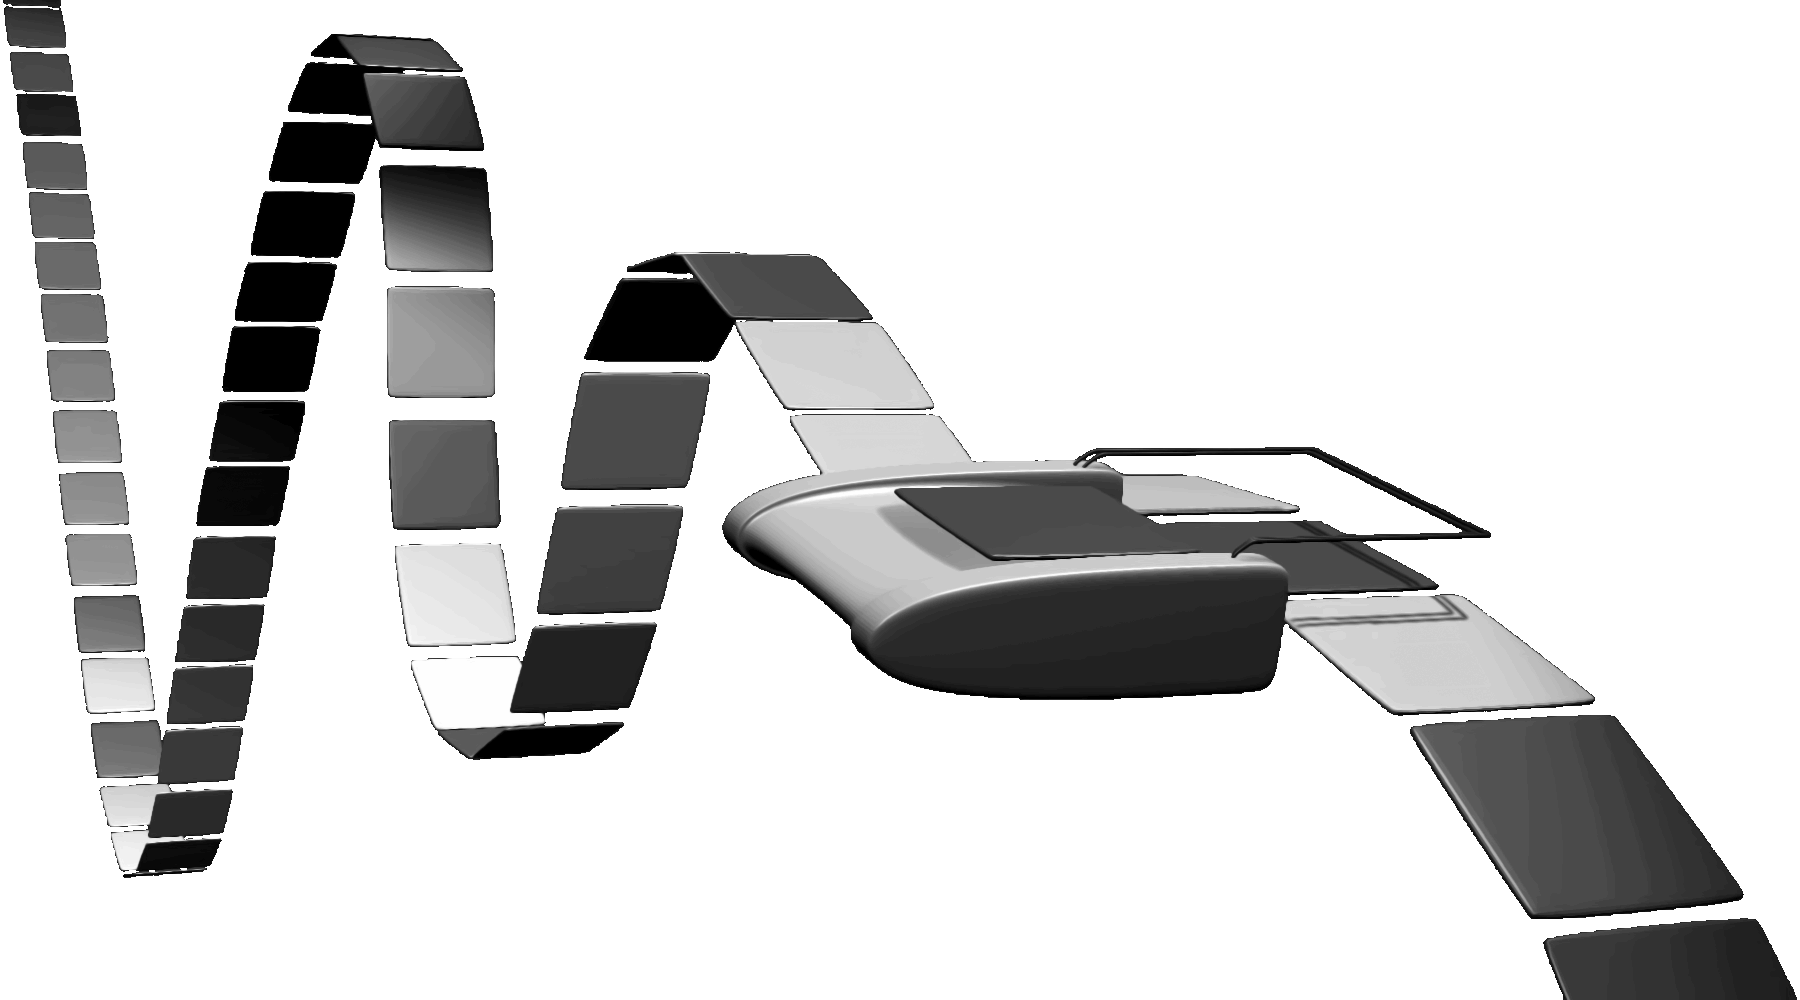
\includegraphics[width=6cm]{turing_machine}
    \caption{An artistic impression of a Turing Machine}
\end{figure}

A formal definition of one is given by Hopcroft and Ullman in their book on theory of automata\cite{IntroToAutomata} as a 7-tuple but, for our purposes, a simpler model with just 4 ingredients shall suffice. Define a Turing Machine as a 4-tuple $(Q, \Gamma, F, \delta)$ where:

\begin{itemize}
    \item $Q$ is a finite, non-empty set of conditions\footnote{Other literature usually refers to these "conditions" as "states". We change the name to avoid confusion with the subtly different notion of "state" we discuss here. That notion is some environment external to a function which affects or is affected by it without being explicitly passed as input.}
    \item $\Gamma$ is a finite, non-empty alphabet of symbols. Each cell on the tape contains one of these symbols.
    \item $F \subset Q$ is a set of {\it final} or {\it accepting} conditions. Upon encountering one of these, the TM finishes its work, leaving the final state of the type to be read off as output.
    \item $\delta: (Q - F) \times \Gamma \rightarrow I$, a mapping from the set of all possible pairs of non-final conditions and symbols to an instruction. It can be thought of as a table of instructions with a column for each condition and a row for each symbol.
    \item $I = \Gamma \times \{L, R\} \times Q$ is the set of all possible instructions this TM could accept. An instruction is a triple of the following things:
        \begin{enumerate}
            \item Replace the symbol in the current cell with any other symbol from the alphabet.
            \item Move the head one space to the left or right.
            \item Change the current (non-final) condition to any condition in Q.
        \end{enumerate}
\end{itemize}

The TM has a head for reading/writing symbols which is positioned over one cell. It operates by reading the value of that cell and feeding that to the function $\delta$ along with its current state and executing the given instruction. This process is repeated until one of the {\it final conditions} from $F$ are reached.

The model of the Turing Machine proved to be a useful advancement. It naturally led to the concept of Turing Completeness which is the ability of a logic system to simulate a Turing Machine\cite{TuringEnigma}. This property is now a widely accepted standard to which a programming language must measure up in order to be considered practically usable. Another advancement is proving the undecidability of the halting problem - the fact that there cannot exist a computer program which can accept another arbitrary program as input and determine whether that program will eventually terminate for a given input.

In relation to programming, the Turing Machine can be thought of as physical representation of the entities present in imperative code, with each cell corresponding to a variable, the alphabet of symbols to the values those variables can take, and each instruction to an assignment statement such as the \code{n = m} in our JavaScript example. The sequence of symbols stored in the tape (along with the currently stored condition), represents the state of the program at a given time.

If the TM is a stateful model of computation, this invites the question of what a stateless one would look like. This is what the $\lambda-calculus$ and combinatory logic we shall look at later provides.

\subsection{Statelessness via Functional Programming}
A computation is merely the mapping of some input to an appropriate output, which exactly matches the notion of a function. A model of one can therefore be built from a system of rules which describes how simpler functions can be combined into larger ones, which is precisely what the combinatory logic developed by Schönfinkel and Curry and the lambda-calculus developed by Alonzo Church does. We shall explore this further in section 3.1 below.

Functional programming is a way of designing languages and writing code which treats functions as data, putting them on the same footing as strings, numbers, etc. This introduces the idea of "higher-order functions", which accept other functions as inputs.

Moreover, languages such as Haskell are said to treat functions as "first-class citizens" - they are declared using the same syntax as concrete pieces of data such as numbers and strings. Indeed, such data can be merely thought of as functions that accept no arguments and so always return a constant value.

\subsection{Functional Languages}
The concept of functional programming is nothing new. The second programming language ever invented, LISP, is functional. LISP was created by MIT's Artificial Intelligence Group to experiment with giving machines the ability to handle declarative as well as imperative statements\cite{RecursiveFunctions}.

A declaration, as opposed to an imperative statement, is one which defines some word or expression as opposed to giving a machine a direct instruction. Such declarations are then used as references by the machine to understand further usage of the defined words/expressions in other points in the program. Expressing a program in terms of such declarations results in the statelessness we talked about earlier because a list of definitions can be written in any order. A list of instructions, in contrast, has to be performed sequentially in order to ensure correct manipulation of state.

This lack of order is taken advantage of in functional programming to break it up into independent units which can be mixed and matched as a coder desires - the kind of modularisation talked about by Graham\cite{OnLisp} and Hughes\cite{WhyFunctional} we mentioned in the introduction.

Since LISP, many other programming languages have been developed which introduced other advancements on top of statelessness. 15 years later, ML became the first statically typed functional language. Static typing is the checking of function signatures at compile time, ensuring that integers, fractions, letters, boolean values, etc are all in their proper place, reducing the likelihood of errors when running a program.

Such type checking requires a formal system of logic, which was built into Church's $\lambda$-calculus by J Roger Hindley and Robin Milner. This type system continues to be used in Haskell, the language with which we shall illustrate the mathematics in this paper. Haskell has a certain syntactic purity not seen in many other languages, requiring no keywords such as \code{def} or \code{function} in order to define a function. To see this, let's look at this code which computes the hypotenuse of a right-angled triangle:
\begin{lstlisting}
    hypot a b = sqrt (a*a + b*b)
\end{lstlisting}
and compare it to the equivalent code in Python:
\begin{lstlisting}
    def hypot(a, b):
        return sqrt(a*a + b*b)
\end{lstlisting}
which has a lot more unnecessary syntactic clutter by way of parentheses, colons, and $return$s. In this way, Haskell's syntax is much closer to mathematical notation and lends itself much better to illustrating the concepts explored in this paper.

Why go functional as opposed to imperative? The reason is productivity. The fields of lambda, combinators, and categories provide a more natural language to express many computational concepts that gives functional code these advantages:
\begin{itemize}
    \item Expressiveness - provide given functionality with terser source code.
    \item Correctness - catch more errors during compile time, reducing run time bugs.
\end{itemize}
As explained earlier, functional programming introduces the idea of functions as first class citizens - treating them as pieces of data on an equal footing with numbers, strings, booleans, etc. This allows functions to be return values and arguments of other functions. In the latter case, those functions which accept other functions as arguments are referred to as being "higher order".

Why is it useful for a function to be higher order? We encounter examples of such functions all the time in mathematics, though they are typically referred to as operators. Consider this Haskell code for numerically approximating the differential operator:
\begin{lstlisting}
    deriv f x = (f (x + h) - f x) / h
        where h = 0.001
\end{lstlisting}
The higher order function is called \code{deriv} and takes 2 arguments, the function $f$ we are differentiating and the point $x$ at which we want the gradient. We also define an arbitrary step size $h$ which regulates the precision of the value we get.

What this means is that, in the functional style, one combines simple functions into more complex ones by putting them together in a similar manner to how one would assemble a Lego model from smaller and smaller modules which are ultimately made out of bricks.

Furthermore, just as Lego parts have these bumps and divots which slot very particularly into one another to hold a model together, the theories of lambda calculus and combinatory logic provide a rigorous framework which describes precisely how larger functions can be built from smaller ones to ensure correctness of a program.
	\section{Lambda-calculus and Combinatory Logic}
\newcommand\reduce{\ \triangleright\ }

In this section on lambda-calculus and combinatory logic (or "lambda" and "CL" as we shall call them for short), we present the ideas of $\beta$-reduction and weak reduction, which are important for evaluating functional expressions. This is based on the material in Hindley and Seldin's excellent book {\it Lambda-calculus and Combinators: an Introduction}~\cite{LambdaAndCombinatorsIntro}. Despite being "an Introduction", the book goes into great detail, including such topics as the undecidability theorem, formal theories, extensionality, and correspondence between lambda and CL in chapters 4 to 9. This is much more than that required for programming, and so we shall restrict ourselves to the most salient points.

\subsection{Function Notation}
Lambda is all about the rules of manipulation of expressions called $\lambda$-terms, which we shall call ``terms''.
To begin with, let us introduce the notation which gives this field its name. We have all seen the more usual mathematical notation for a function:
\begin{equation*}
    f(x,y) = x-y.
\end{equation*}
In the notation of lambda-calculus, we can move the arguments $x,y$ to the right side of the equation to get
\begin{equation*}
    f = \lambda xy.x-y.
\end{equation*}
What this allows one to do is define and call a function without naming it. That is, instead of writing $f(5,3) = 2$, we can directly put
\begin{equation}
    (\lambda xy.x-y)(5,3) = 2.
\end{equation}

\subsection{Currying}
As shown by our \code{deriv} example in section 2.2, one way in which functional programming treats functions as data is by allowing them to be input values for higher order functions. The other way is by returning functions as outputs. In $\lambda$-calculus (and indeed the Haskell language) every multivariate function does this by convention:
\begin{equation}
    \lambda x.\lambda y.E \equiv \lambda xy.E.
\end{equation}
where $E$ is an arbitrary expression in terms of $x$ and $y$\footnote{or no $x$ and $y$ at all in the case of a constant function}. To see this, let's write our function $f$ from the previous section like so:
\begin{equation}
    f=\lambda x.\lambda y.x-y.
\end{equation}
Note how we have separated our arguments $x, y$ such that instead of being passed to $f$ both at once as the pair $(x, y)$, we can put only one in to get a new function which takes the second argument:
\begin{equation}
    f(5)=(\lambda x.\lambda y.x^2-y^2)(3)=\lambda y.3^2-y^2=\lambda y.9-y^2:=f^*.
\end{equation}
We call this new function $f^*$ and can now call it separately from $f$:
\begin{equation}
    f^*(2)=(\lambda y.9-y^2)(2)=9-4=5.
\end{equation}
In other words, we have made the 2-variable function $f$ into a 1-variable one which returns another 1-variable function, which we call $f^*$ in the case $x=3$. This is generalised in lambda to all functions, such that every $n$-variable function actually accepts 1 argument and becomes an $(n-1)$-variable function:
\begin{equation}
    \lambda x_1x_2...x_n.E \equiv \lambda x_1.\lambda x_2...\lambda x_n.E.
\end{equation}
This is called currying, after American logician Haskell Brooks Curry\cite{LambdaAndCombinatorsIntro}. It allows one to perform {\it partial application} of a function, ie supply only some of its arguments. We will see why this is useful by returning to our \code{deriv} example in the next section.

\subsection{An Example of Partial Application}
In Haskell, lambda expressions are written with a backslash instead of a $\lambda$ and an arrow \code{->} instead of a dot. Thus, instead of
\begin{lstlisting}
    hypot = \a b -> sqrt (a*a + b*b)
    
    deriv = \f x -> (f (x+h) - f x) / h
        where h = 0.001
\end{lstlisting}

Now suppose we want to write a new function, \code{deriv2}, to compute the 2\textsuperscript{nd} derivative. If we did not have currying, we would have to write a $\lambda$ expression like so:
\com{Now you use different notations to what was used in this section.
Why you switch to those? Possibly write first in $\lambda$ style and then in Haskel? Reader is still adapting new notations, too soon to jump back. This part can be a good example if explained more slowly and properly}
\begin{lstlisting}
    deriv2 f x = deriv (\y -> deriv f y) x
\end{lstlisting}

This might seem a very neat and tidy way of expressing the second derivative given the first but currying allows us to write this even more succinctly:
\begin{lstlisting}
    deriv2 f x = deriv (deriv f) x
\end{lstlisting}
What we have done here, supplying just one argument of a multivariate function, is called {\it partial application}.\com{is it another name for carrying? You lost me here} This is possible precisely because functions in Haskell are implicitly curried, providing a much more natural way of expressing definitions such as the second derivative being the derivative of the first.
\com{the transition from lambda to Haskel was a bit too abrupt, you need to prepare the reader and first give expressions it both notations. It looks also that the purpose of this seciton is a bit mixed - you have to split in two I think - one to explain the carrying another is to explain how the lambda notation in general translates into Haskel}

\subsection{Left-associativity}
Our final word on notation is that all commas will be eliminated and parentheses minimised. Hence, the usual mathematical expression $f(x,y,z)$ becomes $fxyz$
\com{in the previous section you explained that this should become $\lambda xyz.f$? I.e. here you mean that f is already a lambda expression for a function and it is applied to $x,y,z$ but that is not very clear from the text}. Together with currying, this means function application is left-associative, ie evaluated from left to right thusly\com{here I think one should say that fx means that you feed x into the first argument (as it could also be the last in principle depending on the notations)}:
\begin{equation*}
    fxyz \equiv ((fx)y)z
\end{equation*}
We will endeavour to only use parentheses in cases where function application happens before this left-associativity. An example of this is the case where our variables $x$, $y$, $z$ are instead all functions of another variable $t$:
\begin{equation*}
    f(x(t),y(t),z(t)) \equiv f(xt)(yt)(zt) \equiv ((f(xt))(yt))(zt)
\end{equation*}
where the left expression is the usual one in mathematics, the middle one is what we use in $\lambda$-calculus, and the right expression has the full set of parentheses showing order of application.

\subsection{Building the systems}
Now that we have our notation, it's time to construct our models\com{what do you mean by models - this word is used in too many ways, so needs clarification} which will give us rigorous rules with which to manipulate functions. Since functional programs have no state, their exist no statements which modify it. Instead, a functional program is run by evaluating expressions which consist of $\lambda$-terms and combinators.

Much like Graham's Lisp programs, the set of expressions which we consider valid in $\lambda$ and CL are built from the ground up. If we think of these expressions as Lego\textsuperscript{TM} sets, then the bricks can be thought of as an infinite set of indivisible functions known as atomic constants, denoted by lower case letters. Functions which can be divided into smaller ones will be referred to by capital letters. By restricting function names to single letters like this, we avoid having to put spaces to distinguish them from their inputs, as in our Haskell example \code{hypot a b}.

Imagine you have a set of symbols, called variables. Like atomic constants, these shall be denoted with lower case letters. Then one inductively defines a term as one of the following:
\begin{itemize}
    \item an atom, ie a variable or atomic constant
    \item $(MN)$, the application of one term M to another N
    \item $\lambda x.M$, where x is a variable and M is a term
\end{itemize}
\com{The point does not comes through sufficiently sharply. It sounds repetitive with the previous section, what exactly you are trying to say in 3.4 is not clear.}

\subsection{Manipulating Expressions}
Having defined valid terms, we can now define occurrences, substitutions, contractions, and equivalence, which are key to evaluating functional expressions.
\com{put newly introduced notions in italic}
\com{Give more context to what is going to happen in this section. Logic is lost.}

\subsubsection{Free and Bound Variables}
Consider the following $\lambda$-expression:
\begin{equation*}
    \lambda fg.fx(gy)
\end{equation*}
\com{still unsure how to decode this- this is a function which receives f and g, and then applies f to x and g to y? Is f a function of 2 variables? May be add a bit of an explanation }

Then the variables $f, g$, which are passed as inputs are {\it bound} and those which are not, $x, y$, are called {\it free}\cite{LambdaAndCombinatorsIntro}. The set of free variables of a term $M$ is denoted $FV(M)$. Hence, we have:
\begin{equation*}
    FV(\lambda fg.fx(gy)) = \{f, g\}
\end{equation*}
\com{this looks like a notation thing, which is it in this section? }

\subsubsection{Occurrence}
Let us write $M\ occ\ N$ to say that a term $M$ occurs in $N$. Then, in $\lambda$, the occurrence of one term in another is defined inductively as follows:
\begin{itemize}
    \item $P\ occ\ P$
    \item $P\ occ\ M \lor  P\ occ\ N \iff P\ occ\ (MN)$
    \item $P\ occ\ M \iff P\ occ\ (\lambda x.M)$
\end{itemize}
Note that this means $gx$ does \textbf{not} occur in $fgx$ as function application is left-associative and the term is equivalent to $(fg)x$.

\com{give context - why do we need to define this? Looks a bit random definition without the context.}

\subsubsection{Substitution}
Having defined occurrence, we can now introduce the substitution of $x$ with $P$ in $M$ as the replacement of every free occurrence of $x$ with $P$, changing the names of free variables of $M$ as required to avoid clashes which would change its semantics\cite{LambdaAndCombinatorsIntro}.\com{what is the list below about? You need to introduce it. Are these examples or a definition?}
\begin{itemize}
    \item $[P/x]x \equiv P$
    \item $[P/x]a \equiv a\quad\forall a\not\equiv x$ where a is an atom
    \item $[P/x](MN) \equiv ([P/x]M)([P/x]N)$
    \text{\com{why $x$ cannot appear only when M and N are combined? and not in each of them separately?}}
    \item $[P/x](\lambda x.M) \equiv \lambda x.M$
    \item $[P/x](\lambda y.M) \equiv \lambda y.M$ when $x\notin FV(M)$
    \item $[P/x](\lambda y.M) \equiv \lambda y.[P/x]M)$ when $\neg y\ occ\ P,\ x\in FV(M)$
    \item $[P/x](\lambda y.M) \equiv \lambda z.([P/x][z/y]M)$ when $y\ occ\ P,\ \neg z\ occ\ M,\ x\in FV(M)$
\end{itemize}
With the concept of substitution formally established, we can begin to look into the logic that a functional program performs when evaluating an expression.

\subsubsection{Contraction and Reduction }
\com{what is reduction? I only see contraction explained? Is it the same}
When applying  one function to another, such as $(\lambda x.N)P$, one would expect to be able to simplify the expression by replacing the free instances of $x$ in $N$ with $P$. This intuition is neatly captured in the concept of $\beta$-contraction:
\com{again what is it below? if that is an example introduce it}
\begin{align}
    &(\lambda fgx.fx(gx))(\lambda xy.x)(\lambda xy.x)\\
    &\equiv(\lambda fgx.fx(gx))(\lambda zy.z)(\lambda zy.z)\\
    &\betac (\lambda gx.(\lambda zy.z)x(gx))(\lambda zy.z)\\
    &\betac (\lambda gx.(\lambda y.x)(gx))(\lambda zy.z)\\
    &\betac (\lambda gx.x)(\lambda zy.z)\\
    &\betac (\lambda x.x)
\end{align}

The sequence of steps is as follows:
\begin{enumerate}
    \item In line $(2)$, we change the bound variables $x$ to $z$ in order to avoid clashes with the $x$ in the term $(\lambda fgx.fx(gx))$.
    \item In line $(3)$, we pass the first of the leftmost term's arguments to it, making the substitution $[(\lambda zy.z)/f]$.
    \item In line $(4)$, inside the leftmost expression, we contract $(\lambda zy.z)x \betac (\lambda y.x)$.
    \item In line $(5)$, we make contraction the application of the constant function $(\lambda y.x)(gx) \betac x$.
    \item In line $(6)$, we finally apply the leftmost term to its second argument, also the function $(\lambda zy.z)$. Since $(\lambda gx.x)$ is constant in $g$, this leaves us with the identity function $(\lambda x.x)$.
\end{enumerate}

Beta-reduction is merely a sequence of beta-contractions and is noted with the symbol $\betar$. Hence, a sequence of contractions $J\betac K\betac L\betac M\betac N$ can be written $J\betar N$\com{still unclear why to use the fancy symbol and not just an equal sign?}. Therefore, instead of the lines $(1-7)$ above, one can simply write:
\begin{equation*}
    (\lambda fgx.fx(gx))(\lambda xy.x)(\lambda xy.x) \betar (\lambda x.x)
\end{equation*}

\subsection{Combinatory Logic}
\newcommand\Sc{\textbf S}
\newcommand\Kc{\textbf K}
\newcommand\Ic{\textbf I}

\newcommand\Cc{\textbf C}
\newcommand\Wc{\textbf W}
\newcommand\Bc{\textbf B}
\com{please give a clear definition of combinators here}

The field of combinators 
\com{what is the field of combinators? describe it in some way. Put new notions in italic.}
provides further useful abstractions. Hindley and Seldin motivate the notion as a concise way to state properties of functions\cite{LambdaAndCombinatorsIntro}. Consider, for example, the commutation operator ${\textbf C}$ which swaps the arguments of a binary function:
\begin{equation*}
    \Cc fxy = fyx
\end{equation*}
Once this is defined, one can state a function \com{for a function you would say it is symmetric in its arguments, rather than commutative?} or operator $A$ is commutative by writing
\begin{equation*}
    A = \Cc A
\end{equation*}
The true power of combinators\com{still not clear what or who are the combinators, is C one of them? you did not say that.}, however, lies in their ability to build new functions out of multiple others more concisely \com{more concisely as opposed to what?} by using a "point-free" style, ie without explicitly writing down bound variables with $\lambda$ notation. Mathematicians, in fact, use a combinator when composing functions. Function composition is typically denoted with an empty circle:
\begin{equation*}
    (f \circ g)(x) = f(g(x))
\end{equation*}
In Haskell, a dot is used, allowing us to write our 2\textsuperscript{nd} derivative much more concisely as the composition of two differential operators \com{why C is related to the composition of two functions? Logic is confusing here.}:
\begin{lstlisting}
    deriv2 = deriv.deriv
\end{lstlisting}
Both of these are much shorter than the equivalent $\lambda fgx.f(gx)$ in lambda or \code{\\f g x -> f (g x)} in Haskell. In addition to our commutator $\Cc$ above, some commonly used combinators are:
\begin{itemize}
    \item The identity function $\Ic$ such that $\Ic f = f$. 
    \item The constant function maker $\Kc$ such that $\forall g,\ \Kc fg = f$.
    \item The substitution combinator $\Sc$ where $\Sc fgx = fx(gx)$.
    \item The diagonalisation operator $\Wc$ which turns a function of two arguments into a function of one such that $\Wc fx = fxx$.
    \item The composition operator $\Bc$ where $\Bc fgx = f(gx)$.
    \item The reversed compositor $\Bc'$ where $\Bc' fgx = g(fx)$.
\end{itemize}
\com{what is the significance of the list of those combinators? Is it complete in some sense? Or these are just a few examples? not clear.}
Analogously to lambda's $\beta$-contraction, CL has the notion of weak contraction, denoted by $\weakc$, whereby an expression is simplified through the following substitutions:
\begin{itemize}
    \item $\Ic x\weakc x$
    \item $\Kc xy\weakc x$
    \item $\Sc fgx\weakc fx(gx)$
\end{itemize}

\subsection{Lambda & CL in Practice}
Now that we've developed the ideas of $\lambda$ notation, currying, and combinators, let's see how we might use them in a simple Haskell program.

\subsection{SKI Calculus}
An interesting property of the $\Sc, \Kc, \Ic$ combinators is that they can be used to build any other combinator\com{which are not defined yet, so this statement is hard to appreciate}. While we won't dive into a formal proof of this, the general idea can be illustrated with a couple of simple examples.
Consider the diagonaliser $\Wc$. Through a series of tactical insertions of $\Ic$ and $\Kc$ combinators, we can put its definition in the form of a substitution $\Sc$:
\begin{align}
    \Wc fx&=fxx\\
    &=fx(\Ic x)\\
    &=\Sc f\Ic x\\
    &=\Sc f(\Kc\Ic f)x\\
    &=\Sc\Sc(\Kc\Ic)fx
\end{align}
Thus we obtain $\Wc\equiv\Sc\Sc(\Kc\Ic)$. A slightly more involved problem is expressing the reversed composition operator $\Bc'$ in this way. Firstly, note that it is a commutation of the composition operator, so we break up the problem into two parts:
\begin{equation*}
    \Bc'=\Cc\Bc
\end{equation*}
and begin work on the $\Bc$ combinator:
\begin{align*}
    \Bc fgx&=f(gx)\\
    &=(\Kc fx)(gx)\\
    &=\Sc(\Kc f)gx\\
    &=\Kc\Sc f(\Kc f)gx\\
    &=\Sc(\Kc\Sc)\Kc fgx
\end{align*}
giving us the result $\Bc=\Sc(\Kc\Sc)\Kc$. Now we begin work on the commutation operator:
\begin{align*}
    \Cc fxy&=fyx\\
    &=fy(\Kc xy)\\
    &=\Sc f(\Kc x)y\\
    &=\Bc(\Sc f)\Kc xy\\
    &=\Bc\Bc\Sc f\Kc xy\\
    &=\Bc\Bc\Sc f(\Kc\Kc f)xy\\
    &=\Sc(\Bc\Bc\Sc)(\Kc\Kc)fxy
\end{align*}
where we use our previous definition of $\Bc$ to expedite our arrival at the result $\Cc=\Sc(\Bc\Bc\Sc)(\Kc\Kc)$. Now, through a series of weak contractions, we obtain our final expression:
\begin{align}
    \Bc'&=\Sc(\Bc\Bc\Sc)(\Kc\Kc)\Bc\\
    &\weakc\Bc\Bc\Sc\Bc(\Kc\Kc\Bc)\\
    &\weakc\Bc\Bc\Sc\Bc\Kc\\
    &\weakc\Bc(\Sc\Bc)\Kc\\
    &=\Sc(\Kc\Sc)\Kc(\Sc\Bc)\Kc\\
    &\weakc\Kc\Sc(\Sc\Bc)(\Kc(\Sc\Bc))\Kc\\
    &\weakc\Sc(\Kc(\Sc\Bc))\Kc\\
    &=\Sc(\Kc(\Sc(\Sc(\Kc\Sc)\Kc)))\Kc
\end{align}
It is clear that SKI calculus is not more practical than lambda for all purposes, since this function can simply be written as $\Bc'=\lambda fgx.g(fx)$. It is, however, instructive to see that any function can be represented in this way\com{is it true though? how can you express $\sqrt{x^2+y^2}$ for example?} in principle because it means that any model of computation can be shown to be Turing Complete by showing it can simulate just these 3 combinators.

A particularly fascinating example of this was demonstrated by Michid with the Scala language's type system\cite{ScalaTypeEncoding}. Type systems are usually used to ensure correctness of a program at compile time but, in his article on type level encoding of combinators, Michid used the success or failure of the compilation itself to answer simple yes/no questions about the equivalence of two combinatory terms. To understand how this works, we shall now take a look into functional type systems.

\com{you need a summary at the end of the section, and prepare reader to the next section.}
    \newcommand\ra{\rightarrow}
\section{Type Systems}

The ultimate goal of this paper is to explain the role of monads in asynchronous programming. Before looking at monads, one must understand the type systems which define them. Type systems formally describe the sorts of data with which parts of a program work. They help to check the correctness of a program at compilation, so that it doesn't attempt something nonsensical, such as finding the square root of a string of text or dividing one string by another.

So far, we have trusted that the computations we have built fromLambda expressions and combinators are the building blocks from which one can assemble a generic program but we have been applying them to each other rather indiscriminately, trusting that whatever computations they represent make sense. Type systems prevent coders from compiling programs which attempt to multiply two strings together, for example, or take their square root.

At an abstract level, they do, giving us a new way to think about what a computation really is and how to construct one from the use of just the $\Sc, \Kc, \Ic$ combinators. In the real world, however, we have to manipulate concrete pieces of data such as boolean values, integers, strings, etc, where the type of function becomes very important. 

Neither of these are particularly helpful as they often mean the programmer has made some mistake which is left to the user to deal with. After all, a program shouldn't be written in such a way where one can accidentally attempt to square root a string.

In mathematics, we solve this problem by specifying a domain for each function. . Since they're mappings from one set to another, the destination set, called the range, is also part of a mathematical function definition.

In this section, we shall see how this labelling of functions with input and output sets is essentially the type system devised by Church\cite{LambdaAndCombinatorsIntro}, but also why it is insufficient for programming purposes.

\subsection{Church Typing}

Church defined a type as a single label stuck to each and every $\lambda$ term, signifying the set of possible values it can take. If we have a term $x$ of type $\sigma$, denoted $x^\sigma$, we can't have a term $x^\tau$ where $\sigma\not=\tau$. The system is built from a basis of indivisible {\it atomic} types and defined inductively as follows.
\begin{itemize}
    \item An indivisible {\it atomic} type.
    \item A function type $(\sigma\ra\tau)$ where $\sigma$, $\tau$ are any two types, atomic or other otherwise.
\end{itemize}
Thus, a $\lambda$-term $f^{\sigma\ra\tau}$ can be thought of as the equivalent of the mathematical function declaration $f: \sigma\ra\tau$. This leads to the definition of a typed $\lambda$-term as a more specific version of the one given in section 3.5:
\begin{itemize}
    \item Any typed atom $x^\sigma$ is a typed term.
    \item The application of $M^{\sigma\ra\tau}$ to $N^\sigma$ is a typed term $(MN)^\tau$.
    \item The abstraction $\lambda x^\sigma.M^\tau$ is a typed term $(\lambda x.M)^{\sigma\ra\tau}$.
\end{itemize}
To see some examples of what typed terms look like, let's grab some combinators and analyse their equivalent $\lambda$ expressions.

\subsubsection{Typing Combinators}

Starting with the identity combinator, we define the term $\Ic_\rho$ and apply the type label $\rho$ to our bound variable $x$, which according to the rules above must have the same type label everywhere it occurs:
\begin{equation}
    \Ic_\rho:=\lambda x^\rho.x^\rho=(\lambda x.x)^{\rho\ra\rho}.
\end{equation}
In the rightmost expression, we use the abstraction rule above to deduce that, because we have a function which takes an argument type $\rho$ and returns one of type $\rho$, the overall expression must have the function type $\rho\ra\rho$.

The constant combinator is very similar. We have two variables $x, y$ and assign them the type labels $\rho, \sigma$ respectively. This time, we apply the abstraction rule twice
\begin{align}
    \Kc_{\rho\sigma}:=&\lambda x^\rho y^\sigma.x^\rho
    \\=&\lambda x^\rho.(\lambda y^\sigma.x^\rho)
    \\=&\lambda x^\rho.(\lambda y.x)^{\sigma\ra\rho}
    \\=&(\lambda x.\lambda y.x)^{\rho\ra(\sigma\ra\rho)}
    \\=&(\lambda xy.x)^{\rho\ra\sigma\ra\rho}
\end{align}
where, in line:
\begin{itemize}
    \item $(28)$, we expand the expression to explicitly show its currying.
    \item $(29)$ and $(30)$, we use the abstraction rule on the variable $y$, then $x$.
    \item $(31)$, we contract the expression again. Note that, because arguments are fed into functions one by one due to currying, we implicitly take function types such as
    \begin{equation}
        \rho\ra(\sigma\ra\tau)\equiv\rho\ra\sigma\ra\tau
    \end{equation}
    to be equivalent.
\end{itemize}
Both these examples are rather uninteresting, having only one variable occurrence in the body of the function and only needing the abstraction rule to deduce their types.

For a little more excitement, let's look at the composition combinator $\Bc$ where we are given the typings $x^\rho$ and $f^{\sigma\ra\tau}$.
\begin{equation}
    \Bc_{\rho\sigma\tau}:=\lambda f^{\sigma\ra\tau}gx^\rho.f(gx)
\end{equation}
From the application rule, three deductions can be made. Firstly, the function $f$ maps from $\sigma$ to $\tau$, so the term to which it is applied, $(gx)$, must have type $\sigma$. Secondly, the term it forms, $f(gx)$, must have type $\tau$. In short:
\begin{equation}
    f^{\sigma\ra\tau},\ f(gx)\implies(gx)^\sigma,\ f(gx)^\tau.
\end{equation}
Thirdly, since $x$, of type $\rho$, is mapped by $g$ to a term of type $\sigma$, $g$ must be a function from $\rho$ to $\sigma$. In short:
\begin{equation}
    x^\rho,\ (gx)^\sigma\implies g^{\rho\ra\sigma}.
\end{equation}
This allows us to relabel all the variables in the $\lambda$ expression as shown below.
\begin{equation}
    \Bc_{\rho\sigma\tau}:=\lambda f^{\sigma\ra\tau}g^{\rho\ra\sigma}x^\rho.(f(gx))^\tau
\end{equation}
Finally, we apply the abstraction rule three times, once each for $x, g, f$ in that order, to obtain:
\begin{equation}
    \Bc_{\rho\sigma\tau}:=(\lambda fgx.f(gx))^{(\sigma\ra\tau)\ra(\rho\ra\sigma)\ra\rho\ra\tau}
\end{equation}
A similar flow of logic can be used to deduce the type of any combinator. As an exercise to the reader, the next section

\subsubsection{Typing the $\Sc$ Combinator}
Given the type labellings $x^\rho$, $(gx)^\sigma$, $(fx(gx))^\tau$, deduce the type of variables $f$, $g$, and the term $\Sc_{\rho\sigma\tau}$ in the equation below.
\begin{equation}
    \Sc_{\rho\sigma\tau}:=\lambda fgx^\rho.(fx(gx)^\sigma)^\tau
\end{equation}
You will need to use the application rule as well as the abstraction rule.

\subsection{Polymorphic Typing}

In contrast to Church's prescriptive type system, which assigns a type to every expression before using it, Curry developed a descriptive type system, which deduces the type of an expression while evaluating it. To see why this is useful, consider the simple case of the identity function. According to Church's system, one would separately have to declare combinators $\Ic_\rho, \Ic_\sigma, \Ic_\tau$ for every single type $\rho, \sigma, \tau$ on which one wants to apply it.

\begin{lstlisting}
    id_int :: Int -> Int
    id_int x = x
    
    id_str :: String -> String
    id_str x = x
    
    id_bool :: Boolean -> Boolean
    id_bool x = x
\end{lstlisting}

Polymorphism is the ability of a given expression to take on different types in different contexts. In the case of the identity combinator, this means one can make a single function declaration which works for all types.

\begin{lstlisting}
    id :: a -> a
    id x = x
\end{lstlisting}

\subsection{Type Classes}
\subsection{Type Constructors} 
    \section{Monads}
Up until now, we have shunned state as being as being a superfluous entity for the conception of an algorithm. We treated every computer program as the evaluation of a single expression, typically a complex one built from many smaller, simpler ones like Lego bricks.

This is, of course, a simplification. The modelling program as a function is all well and good for a one which does nothing more than perform a single calculation, deterministically mapping each given user input to a certain output. Most programs, however, have to interact with the outside world in a more persistent manner. They have to present an interface to the user that can be used to invoke multiple calculations or communicate with another computer over a network.

Surely statefulness cannot be avoided here? The outside world is, after all, inherently stateful and, furthermore, unreliable. Networks can fail, computers can crash, errors can creep in.

Category theory comes to the rescue by providing a convenient structure known as the monad. There are  as many different kinds of state as there are environments in which a program can run and a specific monad type can be designed for each one. As a result of this, monads provide a highly versatile, unified interface to computation that can encapsulate any kind of real world interaction ranging from basic text input/output on a command line to downloading data from a web server.

\subsection{Definition}
\begin{lstlisting}
    class Monad m where
        return :: a -> m a
        (>>=) :: m a -> (a -> m b) -> m b
\end{lstlisting}
\subsection{Monad Laws}
\begin{itemize}
    \item Left identity: \texttt{return x >>= f = f x}
    \item Right identity: \texttt{x >>= return = x}
    \item Associativity: \texttt{(x >>= f) >>= g = x >>= ($\backslash$y -> f y >>= g)}
\end{itemize}


To get a taste of how monads work, we shall take a look at the simplest one - \code{Maybe}.
\hidden{
    \subsection{Branching}
	Some types of computation may return multiple values from a single one. In such cases, a list data type is used as a container for all these values. This branching of one value into many can be thought of as a form of statefulness and, as such, lists can be thought of as monads. In order to implement them as such, one has to define the \texttt{return} and \texttt{>>=} as described earlier.
}
\subsection{Error Handling}
How can one use a static type system to encode computations which may have errors potentially creep in, or undefined values? In Haskell, this is done with the $Maybe$ monad.
\begin{lstlisting}
    data Maybe a = Just a | Nothing
\end{lstlisting}
\subsection{Asynchronicity}
Asynchronous operations are ones which happen independently of a program's normal flow. This happens when a web application requests data from a different web service, such as an Overleaf user taking the option to log in via their institution. If you're a King's student, for example, that web service is Microsoft Online.
The reason why a different flow is involved is because two computers are involved, with one making an HTTP request to the other. Since this requires communication over a network, problems may arise such as connectivity issues or server errors.
So if the data from the server is represented in your program by a type $\sigma$ one can't simply extract it with a function whose return type is also $\sigma$ because that implies a guaranteed result. Instead, we need a structure which encapsulates the possibility of failure, much like the \code{Maybe} monad. Luckily for us, some clever people have already created such structures, known as promises or futures. Both essentially function the same way, having values which fall into one of two camps: a success, along with the desired data; or a failure, typically with some sort of error message.


    \section{Appendix}
\subsection{}
    
	\bibliographystyle{alpha}
    \bibliography{references}
\end{document}
